\documentclass[11pt,a4paper]{article}

%% ============================================================================
%% The Forced Derivation of K₄ from Logical Distinction
%% Companion paper for TYPES / LICS / CSL submission
%% ============================================================================

\usepackage[utf8]{inputenc}
\usepackage[T1]{fontenc}
\usepackage{unicode-math}
\usepackage{libertine}
\usepackage{inconsolata}
\usepackage[margin=2.5cm]{geometry}
\usepackage{amsmath,amsthm}
\usepackage{hyperref}
\hypersetup{colorlinks=true,linkcolor=blue!60!black,citecolor=blue!60!black,urlcolor=blue!70!black}
\usepackage{enumitem}
\usepackage{tikz}
\usetikzlibrary{positioning,arrows.meta,calc}
\usepackage{newunicodechar}

%% Unicode mappings (subset needed for code excerpts)
\newunicodechar{¬}{\ensuremath{\neg}}
\newunicodechar{×}{\ensuremath{\times}}
\newunicodechar{∀}{\ensuremath{\forall}}
\newunicodechar{→}{\ensuremath{\to}}
\newunicodechar{≡}{\ensuremath{\equiv}}
\newunicodechar{≠}{\ensuremath{\neq}}
\newunicodechar{⊥}{\ensuremath{\bot}}
\newunicodechar{⊤}{\ensuremath{\top}}
\newunicodechar{⊎}{\ensuremath{\uplus}}
\newunicodechar{ℕ}{\ensuremath{\mathbb{N}}}
\newunicodechar{λ}{\ensuremath{\lambda}}
\newunicodechar{ω}{\ensuremath{\omega}}
\newunicodechar{₀}{\ensuremath{_0}}
\newunicodechar{₁}{\ensuremath{_1}}
\newunicodechar{₂}{\ensuremath{_2}}
\newunicodechar{₃}{\ensuremath{_3}}
\newunicodechar{₄}{\ensuremath{_4}}
\newunicodechar{⁺}{\ensuremath{^+}}
\newunicodechar{≤}{\ensuremath{\le}}
\newunicodechar{≺}{\ensuremath{\prec}}
\newunicodechar{≗}{\ensuremath{\circeq}}

%% Theorem environments
\newtheorem{theorem}{Theorem}[section]
\newtheorem{lemma}[theorem]{Lemma}
\newtheorem{proposition}[theorem]{Proposition}
\newtheorem{corollary}[theorem]{Corollary}
\theoremstyle{definition}
\newtheorem{definition}[theorem]{Definition}

%% Code display
\usepackage{listings}
\lstset{
  language=,
  basicstyle=\small\ttfamily,
  keywordstyle=\bfseries,
  breaklines=true,
  columns=fullflexible,
  literate={→}{{$\to$}}1 {∀}{{$\forall$}}1 {≡}{{$\equiv$}}1 {≠}{{$\neq$}}1
           {⊥}{{$\bot$}}1 {⊤}{{$\top$}}1 {⊎}{{$\uplus$}}1 {ℕ}{{$\mathbb{N}$}}1
           {λ}{{$\lambda$}}1 {¬}{{$\neg$}}1 {×}{{$\times$}}1 {≗}{{$\circeq$}}1
           {≤}{{$\le$}}1 {≺}{{$\prec$}}1 {⁺}{{$^+$}}1 {ω}{{$\omega$}}1
           {₀}{{$_0$}}1 {₁}{{$_1$}}1 {₂}{{$_2$}}1 {₃}{{$_3$}}1 {₄}{{$_4$}}1,
  frame=single,
  framexleftmargin=2pt,
  xleftmargin=6pt,
  xrightmargin=4pt,
  aboveskip=8pt,
  belowskip=8pt,
}

\title{The Forced Derivation of $K_4$ from Logical Distinction\\[0.3em]
\large A Machine-Verified Eliminative Chain in Agda}
\author{Johannes Michael Wielsch}
\date{April 2026}

\begin{document}
\maketitle

%% ============================================================================
\begin{abstract}
We present a self-contained derivation, mechanically verified in Agda under
\texttt{-{}-safe -{}-without-K}, that the complete graph $K_4$ is the unique
fixpoint of an eliminative filter starting from a single axiom: the existence
of a distinction.

A \emph{distinction} is a type with two provably unequal inhabitants and
a coverage guarantee that every element equals one of them.
From this datum alone, we derive:
(i)~exactly four mutually distinct endomorphisms,
(ii)~a well-founded drift hierarchy via universe-level iteration,
(iii)~a presentation fixpoint collapsing every admissible observable to a
canonical base,
and (iv)~the complete graph on four vertices as the unique structure
surviving all constraints.

No postulate, no axiom, and no external import beyond
\texttt{Agda.Primitive} is used.  The proof artifact is a single literate
Agda file; this paper is its narrative extract.
\end{abstract}

%% ============================================================================
\section{Introduction}
\label{sec:intro}

The question this paper addresses is narrow: given the weakest possible
starting point---a type with exactly two distinguishable elements---what
combinatorial structure does self-consistency force?

The answer is $K_4$, the complete graph on four vertices.  The derivation
proceeds by elimination: at each stage, every alternative that fails an
internal consistency requirement is destroyed, and the unique survivor
is carried forward.  The elimination chain has five links:

\begin{enumerate}[nosep]
  \item Distinction forces four endomorphisms.
  \item Level iteration forces a well-founded drift hierarchy.
  \item Acyclicity forces every drift chain to terminate.
  \item Observables collapse to a canonical presentation fixpoint.
  \item The fixpoint forces $K_4$ as the unique surviving graph.
\end{enumerate}

Each link is machine-checked.  The Agda source is compiled under
\texttt{-{}-safe -{}-without-K}, which prohibits postulates, axiom K,
and any escape from constructive type theory.  The entire development
uses no library beyond \texttt{Agda.Primitive} for universe levels.

\paragraph{Related work.}
Exhaustive classification of finite structures under algebraic constraints
has a long history (Cayley's enumeration of groups, Burnside's lemma,
modern computational algebra).  The novelty here is not classification
\emph{per se} but the demonstration that a single binary distinction,
iterated through universe levels, forces exactly one graph through purely
type-theoretic means.  The work closest in spirit is the programme of
homotopy type theory \cite{hottbook}, which also derives geometric
structure from type-theoretic primitives, though the methods and targets differ.

%% ============================================================================
\section{The Distinction Axiom}
\label{sec:distinction}

\begin{definition}[Distinction]
A \emph{distinction} is a record consisting of:
\begin{itemize}[nosep]
  \item a carrier type $S : \mathsf{Set}$,
  \item two elements $\ell, r : S$,
  \item a separation proof $\ell \neq r$,
  \item a coverage function $\mathit{cover} : (x : S) \to (x \equiv \ell) \uplus (x \equiv r)$.
\end{itemize}
\end{definition}

In Agda:

\begin{lstlisting}
record Distinction : Set1 where
  field
    S     : Set
    l     : S
    r     : S
    l!=r  : l != r
    cover : (x : S) -> (x == l) + (x == r)
\end{lstlisting}

Coverage is the critical field.  Without it, $S$ could contain hidden
elements unreachable by $\ell$ and $r$, and the classification that
follows would be incomplete.  With it, every element is provably one of
two values, and every function $S \to S$ is determined by its action on
$\ell$ and $r$.

%% ============================================================================
\section{Four-Case Endomorphism Classification}
\label{sec:four-cases}

\begin{theorem}[Classification]
\label{thm:classify}
Let $d$ be a distinction.  Every endomorphism $f : S \to S$ is
classified by one of exactly four cases:
\[
\mathit{EndoCase} \;=\; \mathit{constL} \mid \mathit{constR} \mid \mathit{id} \mid \mathit{dual}
\]
The classification is:
\begin{itemize}[nosep]
  \item \textbf{sound}: $\mathit{interpret}(\mathit{classify}(f)) \circeq f$,
  \item \textbf{injective}: $\mathit{interpret}(c) \circeq \mathit{interpret}(c') \;\Rightarrow\; c \equiv c'$,
  \item \textbf{unique}: $\mathit{interpret}(c) \circeq f \;\Rightarrow\; c \equiv \mathit{classify}(f)$.
\end{itemize}
\end{theorem}

\begin{proof}[Proof sketch]
Classification dispatches on $\mathit{cover}(f(\ell))$ and
$\mathit{cover}(f(r))$, yielding $2 \times 2 = 4$ branches.  Soundness
follows by case analysis and symmetry of equality.  Injectivity is proved
by a $4 \times 4$ exhaustion: for each pair of distinct cases, the
assumption $\mathit{interpret}(c) \circeq \mathit{interpret}(c')$ produces a
contradiction via $\ell \neq r$.  Uniqueness combines soundness and
injectivity.  All three are verified by Agda. \qed
\end{proof}

The key consequence: the endomorphism monoid of any distinction is
\emph{exactly} four elements.  Not three (which would orphan a case),
not five (which would require a third boundary value).

\begin{figure}[h]
\centering
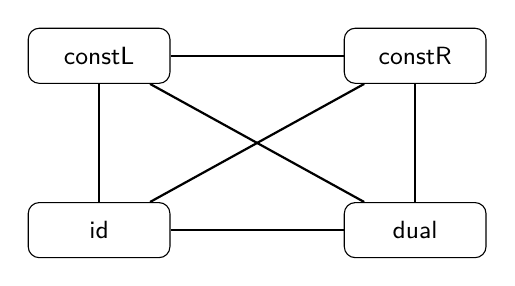
\begin{tikzpicture}[>=Latex, node distance=1.8cm, every node/.style={draw, rounded corners, minimum width=1.8cm, minimum height=0.7cm, font=\small\sffamily}]
  \node (cL) {constL};
  \node[right=2.2cm of cL] (cR) {constR};
  \node[below=1.5cm of cL] (id) {id};
  \node[right=2.2cm of id] (du) {dual};

  \draw[thick] (cL) -- (cR);
  \draw[thick] (cL) -- (id);
  \draw[thick] (cL) -- (du);
  \draw[thick] (cR) -- (id);
  \draw[thick] (cR) -- (du);
  \draw[thick] (id) -- (du);
\end{tikzpicture}
\caption{The four endomorphism cases and their pairwise distinctness.  Every pair is connected because every pair is provably $\neq$.  This is $K_4$.}
\label{fig:k4-endo}
\end{figure}

%% ============================================================================
\section{Drift Hierarchy and Acyclicity}
\label{sec:drift}

Classification applies not only within a single distinction but
\emph{across universe levels}.  Applying the classification functor to
its own output produces a tower of drift states, one per level of the
type hierarchy.

\begin{definition}[Drift State]
A drift state packages a distinction at a given universe level together
with its derived structure.  The step function lifts a drift state one
level higher.
\end{definition}

\begin{definition}[Reachability]
Strict reachability $s \prec^+ t$ is the transitive closure of the
step relation.  Reflexive reachability $s \preceq t$ adds the identity.
\end{definition}

\begin{theorem}[Ranking forces acyclicity]
\label{thm:acyclic}
If there exists a rank function $\mathit{rank} : \mathit{DriftState} \to
\mathbb{N}$ such that each step strictly increases the rank, then the
drift hierarchy is acyclic: no state is strictly reachable from itself.
\end{theorem}

\begin{proof}[Proof sketch]
A cycle $s \prec^+ s$ forces $\mathit{suc}(\mathit{rank}(s)) \le
\mathit{rank}(s)$ by monotonicity, which is impossible in~$\mathbb{N}$.
Verified as \texttt{law11-1-ranked-acyclic} in the Agda source.
\qed
\end{proof}

%% ============================================================================
\section{Presentation Fixpoint}
\label{sec:fixpoint}

\begin{definition}[Presentation]
A presentation of the endomorphism classification is a type $X$ together
with maps $\mathit{interpret} : X \to (S \to S)$ and
$\mathit{classify} : (S \to S) \to X$ satisfying soundness and
injectivity.
\end{definition}

\begin{theorem}[Presentation collapse]
\label{thm:presentation}
Every presentation is isomorphic to $\mathit{EndoCase}$.  In particular,
any admissible observable on proofs factors through the canonical
four-element base.
\end{theorem}

This fixpoint property means that no matter how the four-element
classification is re-encoded or re-presented, the underlying structure is
invariant.  There is no presentation freedom.

%% ============================================================================
\section{$K_4$ as Unique Survivor}
\label{sec:k4}

\begin{definition}[Graph]
A graph is a type $V$ of vertices with a symmetric, irreflexive edge
relation $\mathit{Edge} : V \to V \to \mathsf{Set}$.
\end{definition}

\begin{definition}[Canonical $K_4$]
The canonical $K_4$ has $V = \mathit{EndoCase}$ and
$\mathit{Edge}(a,b) = (a \neq b)$.
\end{definition}

Since all four endomorphism cases are mutually distinct
(Section~\ref{sec:four-cases}), every pair is connected.  The result is
the complete graph on four vertices.

\begin{theorem}[Presentation uniqueness]
\label{thm:k4-unique}
Every $K_4$ graph presentation---any alternative vertex type $X$ equipped
with a bijection to $\mathit{EndoCase}$---produces a graph isomorphic to
the canonical $K_4$.
\end{theorem}

\begin{proof}[Proof sketch]
The bijection transports the edge relation (inequality) faithfully.
Distinctness is invariant under renaming.  Verified as
\texttt{law13-1-presentation-iso} in the source.
\qed
\end{proof}

\begin{figure}[h]
\centering
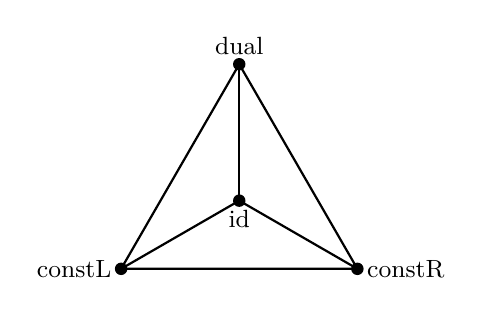
\begin{tikzpicture}[scale=1.5]
  \coordinate (A) at (0,0);
  \coordinate (B) at (2,0);
  \coordinate (C) at (1,1.732);
  \coordinate (D) at (1,0.577);
  \draw[thick] (A) -- (B) -- (C) -- cycle;
  \draw[thick] (A) -- (D);
  \draw[thick] (B) -- (D);
  \draw[thick] (C) -- (D);
  \foreach \p in {A,B,C,D} \fill (\p) circle (1.5pt);
  \node[left] at (A) {\small constL};
  \node[right] at (B) {\small constR};
  \node[above] at (C) {\small dual};
  \node[below] at (D) {\small id};
\end{tikzpicture}
\caption{$K_4$: the complete graph on the four endomorphism cases.}
\label{fig:k4-tetrahedron}
\end{figure}

%% ============================================================================
\section{The Elimination Chain}
\label{sec:chain}

The full derivation is summarized in Table~\ref{tab:chain}.

\begin{table}[h]
\centering
\small
\renewcommand{\arraystretch}{1.3}
\begin{tabular}{@{}r l p{4.2cm} p{4.2cm}@{}}
\hline
\textbf{\#} & \textbf{Survivor} & \textbf{Why it survives} & \textbf{Eliminated} \\
\hline
1 & Distinction ($D_0$) & Binary separation with coverage. & Vacuous carriers, partial classifications. \\
2 & Four endomorphisms & $2 \times 2 = 4$ cases, mutually distinct. & $K_1$, $K_2$, $K_3$ (orphan cases). \\
3 & Drift acyclicity & Ranking forces well-foundedness. & Cyclic hierarchies, infinite descent. \\
4 & Presentation fixpoint & Observables factor through canonical base. & Non-canonical representations. \\
5 & $K_4$ & Unique complete graph on four vertices. & All proper subgraphs and supergraphs. \\
\hline
\end{tabular}
\caption{The eliminative chain from distinction to $K_4$.}
\label{tab:chain}
\end{table}

%% ============================================================================
\section{Formal Environment}
\label{sec:formal}

The development is a single literate Agda file (\texttt{FirstDistinction.lagda.tex}),
approximately 25{,}000 lines, compiled under:

\begin{lstlisting}
{-# OPTIONS --safe --without-K #-}
module FirstDistinction where
open import Agda.Primitive using (Level; lzero; lsuc; _+_; Setw)
\end{lstlisting}

\noindent No standard library.  No postulates.  No axiom K.  All
infrastructure---equality, negation, decidability, coproducts, natural
numbers, ordering---is built from scratch within the file.

The \texttt{-{}-safe} flag forbids \texttt{postulate}, \texttt{TERMINATING},
and other escape hatches.  The \texttt{-{}-without-K} flag forbids
Streicher's axiom K, ensuring compatibility with homotopy type theory.

The proof artifact is available at
\url{https://github.com/de-johannes/Void}.

%% ============================================================================
\section{Discussion}
\label{sec:discussion}

The result is a purely combinatorial classification theorem: the only
graph that survives the eliminative filter forced by a single distinction
is $K_4$.  The derivation introduces no free parameter and makes no
appeal to geometry, physics, or model-theoretic semantics.

Several questions remain open for the type-theory community:

\begin{itemize}[nosep]
  \item Can the exhaustive classification be sharpened to a single
        categorical universal property?
  \item What is the precise relationship between the drift hierarchy
        and ordinal notations in proof theory?
  \item Does the presentation fixpoint admit a formulation in terms of
        initial algebras or terminal coalgebras?
  \item Can the result be reproduced in alternative proof assistants
        (Lean~4, Coq) to confirm independence from Agda-specific
        features?
\end{itemize}

The companion book~\cite{wielsch2026first} extends the derivation into
arithmetic and spectral analysis, but those extensions are not part of
the present claim.  This paper concerns only the formal chain from
distinction to~$K_4$.

%% ============================================================================
\section{Conclusion}
\label{sec:conclusion}

We have shown that a single binary distinction---a type with two provably
unequal, covering elements---forces, through an eliminative chain
verified in Agda under \texttt{-{}-safe -{}-without-K}, exactly four
mutually distinct endomorphisms, a well-founded drift hierarchy, a
canonical presentation fixpoint, and the complete graph $K_4$ as the
unique survivor.

No alternative survives at any stage.  The derivation is not a choice
among models but the execution of a filter that destroys every unstable
alternative.  The Agda source serves as both proof and artifact.

\paragraph{Acknowledgements.}
This paper extracts the formal core of the book \emph{First Distinction:
A Logical Ontology of Distinction}. The full development is available as
a literate Agda file at \url{https://github.com/de-johannes/Void}.

\begin{thebibliography}{9}
\bibitem{hottbook}
  The Univalent Foundations Program,
  \emph{Homotopy Type Theory: Univalent Foundations of Mathematics},
  Institute for Advanced Study, 2013.

\bibitem{wielsch2026first}
  J.\,M.~Wielsch,
  \emph{First Distinction: A Logical Ontology of Distinction},
  2026.
  \url{https://github.com/de-johannes/Void}
\end{thebibliography}

\end{document}
